\documentclass[border=10pt]{standalone}
\usepackage{tikz}
\usetikzlibrary{arrows.meta, shapes, positioning, calc}

\begin{document}
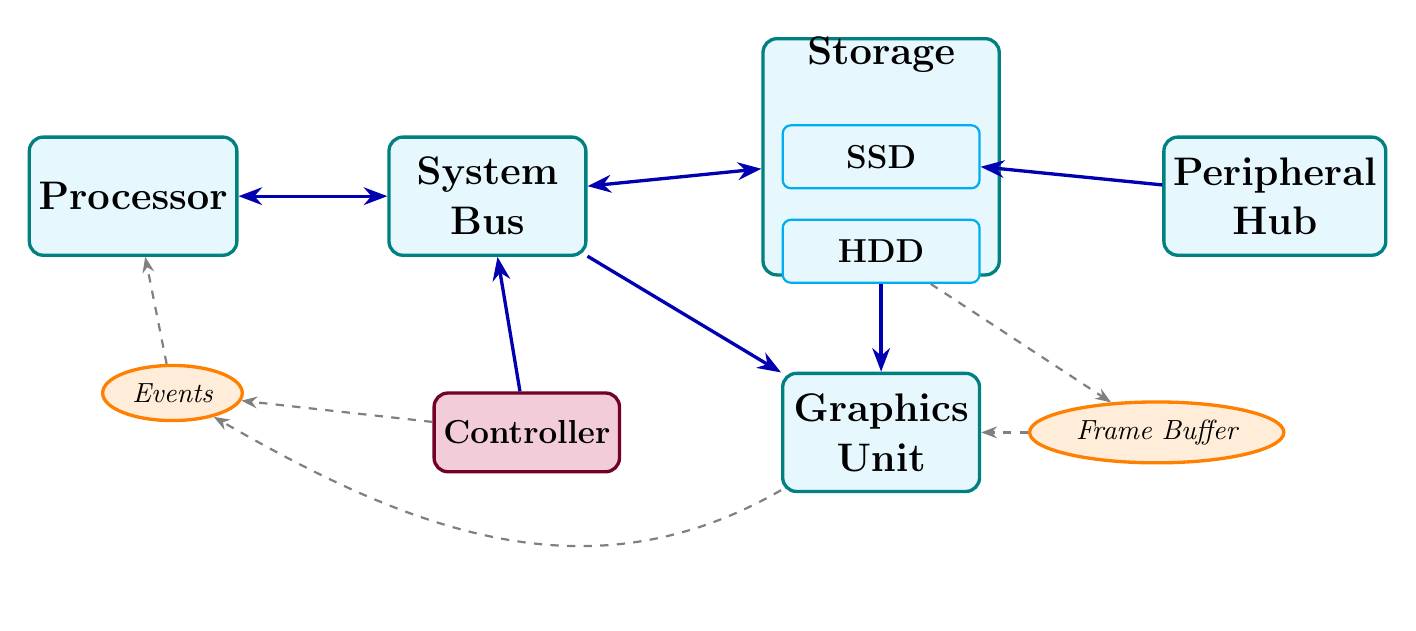
\begin{tikzpicture}[
    node distance=2cm,
    component/.style={rectangle, rounded corners=5pt, draw=teal, very thick, fill=cyan!10, minimum width=2.5cm, minimum height=1.5cm, align=center, font=\Large},
    storage/.style={rectangle, rounded corners=5pt, draw=teal, very thick, fill=cyan!10, minimum width=3cm, minimum height=3cm, align=center},
    subcomponent/.style={rectangle, rounded corners=3pt, draw=cyan, thick, fill=cyan!10, minimum width=2.5cm, minimum height=0.8cm, align=center, font=\large},
    controller/.style={rectangle, rounded corners=5pt, draw=purple!60!black, very thick, fill=purple!20, minimum width=2cm, minimum height=1cm, align=center, font=\large},
    event/.style={ellipse, draw=orange, very thick, fill=orange!15, minimum width=1.5cm, minimum height=0.7cm, align=center, font=\itshape},
    arrow/.style={-{Stealth[length=3mm]}, very thick, blue!70!black},
    doublearrow/.style={{Stealth[length=3mm]}-{Stealth[length=3mm]}, very thick, blue!70!black},
    dashedarrow/.style={-{Stealth[length=2mm]}, thick, gray, dashed}
]

% Main components
\node[component] (processor) at (0,0) {\textbf{Processor}};
\node[component] (bus) at (4.5,0) {\textbf{System}\\\textbf{Bus}};
\node[storage] (storage) at (9.5,0.5) {};
\node[component] (peripheral) at (14.5,0) {\textbf{Peripheral}\\\textbf{Hub}};

% Storage label and subcomponents
\node[font=\Large] at (9.5,1.8) {\textbf{Storage}};
\node[subcomponent] (ssd) at (9.5,0.5) {\textbf{SSD}};
\node[subcomponent] (hdd) at (9.5,-0.7) {\textbf{HDD}};

% Controller and Graphics Unit
\node[controller] (controller) at (5,-3) {\textbf{Controller}};
\node[component] (graphics) at (9.5,-3) {\textbf{Graphics}\\\textbf{Unit}};

% Event nodes
\node[event] (events) at (0.5,-2.5) {\textit{Events}};
\node[event] (framebuffer) at (13,-3) {\textit{Frame Buffer}};

% Main connections
\draw[doublearrow] (processor) -- (bus);
\draw[doublearrow] (bus) -- (storage);

% Controller connections
\draw[arrow] (controller) -- (bus);
\draw[arrow] (bus) -- (graphics);
\draw[arrow] (hdd) -- (graphics);

% Peripheral to SSD
\draw[arrow] (peripheral) -- (ssd);

% Dashed event connections
\draw[dashedarrow] (events) -- (processor);
\draw[dashedarrow] (controller) -- (events);
\draw[dashedarrow] (graphics) to[out=210,in=330] (events);
\draw[dashedarrow] (hdd) -- (framebuffer);
\draw[dashedarrow] (framebuffer) -- (graphics);

\end{tikzpicture}
\end{document}
